% !TeX spellcheck = da_DK
\subsection{Komparator}
\subsubsection{Teori og design}
Som nævnt i afsnit \ref{Komparatorafsnit} på side \pageref{Komparatorafsnit} anvendes en komparator til at sammenligne to inputspændinger. I dette tilfælde vil komparatorens output blive tilkoblet hhv. en LED-diode eller/og vibrator, en modstand og den positive spændingsforsyning ($+V_{cc}$). I komparatorens inverterende terminal skal outputtet fra forrige blok tilsluttes. Inputtet til den ikke-inverterende terminal skal være reference spændingen, hvilket anvendes til at angive de beregnede tærskelværdier. Komparatoren kan derfor have to forskellige outputs afhængig af inputspændingen. Hvis inputsignalet er mindre end den beregnede tærskelværdi, vil outputtet være $0V$, og dioderne og vibratoren vil ikke aktiveres. Er inputtet højere end tærskelværdien, vil outputtet svare til jord, da strømmen fra $+V_{cc}$ vil løbe igennem komparatoren og derefter til jord. Derved opnås et spændingsfald over den positive og negative pol for LED-dioden og vibratoren på en værdi, der ligger over det minimale spændingsfald, der kræves for en aktivering. LED-dioderne og vibratorerne vil derved blive aktiveret og give feedback til patienten. \\

\noindent\textbf{Visuel komparator kredsløb} \\
Til den visuelle del af komparator kredsløbet bruges der LED-dioder. Diodernes katode skal tilkobles komparatorens output, hvorimod dens anode skal tilkobles $+V_{cc}$. For aktivering af LED-dioderne vil der blive anvendt seks komparatorer, da der ifølge kravspecifikationerne i afsnit \ref{KomparatorAfs} på side \pageref{KomparatorAfs} er fem forskellige stadier for aktivering Der skal midlertidig bruges seks da den ene stadie både har positive og negative tærskelværdier og derfor skal der bruge to komparatorere til dette stadie. Tærskelværdierne for disse kan både implemeteres som to spændingstræer eller som otte spændingsdelere. Der er fordele og ulemper ved begge metoder. Det vælges at bruge otte spændingsdelere, hvor fire indgår i to vindues-komparatorere og fire i normale komparatorere. 
Dette design bliver valgt til fordel for to spændingtræer, da modstandene i et spændingstræ har påvirkning på hinanden og derved kan der ske ændringer i alle tærskelværdier, hvis én af modstandene ikke fungere ideelt. For at sikre dette ikke sker, brugs der derved en spændingsdeler for hver tærskelværdi som kan ses på figur \figref{fig:komparator_visuel}.
Derudover bruges der en spændingsreference $+V_{ref}$ på $2.5$V og  seks modstande (R$15$-R$20$) mellem LED-dioderne og $+V_{cc}$ for at beskytte LED-dioderne mod for høj strømstyrke og undgå, at batteriet drænes. Desuden bliver der placeret  dioder (D$7$ - D$10$) ved hver af de to operations forstærkere(TL$081$) i vindues-komparationen. Dette gøres for at adskille de to operations forstærkere ellers ville de påvirke hinanden og vindues-komparatoren vil derved ikke fungere som ønsket.  
\begin{figure}[H]
	\centering
	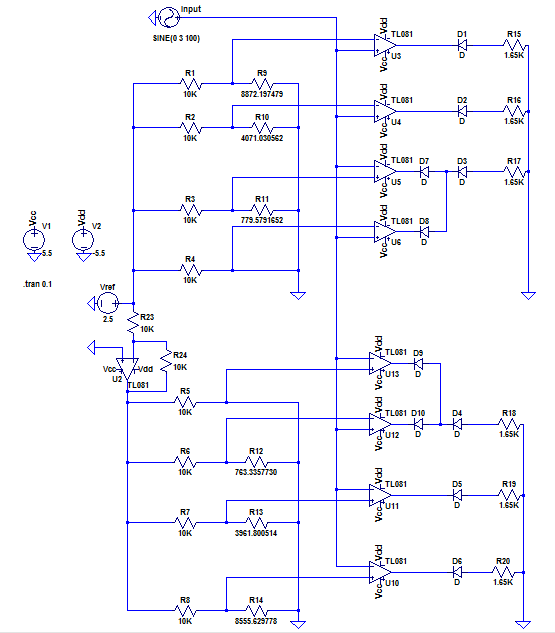
\includegraphics[scale=1.0]{figures/cProblemloesning/komparator_visuel.PNG}
	\caption{Figuren er et overblik over komparator kredsløbet for den visuelle del lavet i LTspice. Kredsløbet består af to dele; en for hældning i positiv retning og en for hældning i negativ retning. Hver del er består af en vindues-komparator og to normale komparatorere. Der er en inverterende forstærker for at gøre referencespændingen negativ, så hældning i den negative retning kan dedekteres}
	\label{fig:komparator_visuel}
\end{figure}

%%%%%%%%%%%%%%%%%%%%%%%%%%%%%%%%%%%%%%%%%%%%%%%%%%%%%%%%%%%%%%%

\noindent\textbf{Beregning af tærskelværdier og tilhørende R$1$-R$14$ modstande for aktivering af LED-dioder} \\
Inputsignalet fra forrige blok, som er tilpasningsblokken, vil være et signal, der ligger imellem -$2.2168$V og $2.2602$V jævnført afsnit \ref{KomparatorAfs} på side\pageref{KomparatorAfs}. Ifølge systemets funktionelle krav i afsnit \ref{FunkKrav} på side \pageref{FunkKrav} ønskes det, at LED-dioderne skal lyse ved en bestemt kropshældning, dvs. ved en bestemt tærskelværdi. %Disse tærskelværdier sættes ud fra to punkter; det maksimale teoretiske signal  ved $25^{\circ}$ $4.0662$, og en tilgængelig spændingsreference, der kan sørge for en fast spænding til spændingstræet. 
Tærskelværdierne er som jævnført afsnit \ref{KomparatorAfs} udregnet til at være:
\begin{itemize}
\item $2^{\circ}$ = $0.1808$V
\item -$2^{\circ}$ = -$01773$V
\item $8^{\circ}$ = $0.7233$V
\item -$8^{\circ}$ = -$0.7094$V
\item $13^{\circ}$ = $1.1753$V
\item -$13^{\circ}$ = -$1.1527$V
\item $25^{\circ}$ = $2.2602$V
\item -$25^{\circ}$ = -$2.2168$V
\end{itemize}}

Der vælges en  spændingsreference, som består af en regulator så den kan levere $2.5$V til komparatorkredløbet. Spændingsreferencen indgår som del af en spændingsdeler og benyttes for at holde en fast referencespænding, da spændingen ellers vil falder over tid, som det ville være tilfældet hvis, der blev anvendt et batteri som spændingsforsyning. For at det er muligt at bruge den $2.5$V spændingsforsyning til de negative tærskelværider bruges en inverterende forstærker med et gain på en som kan ses på figur \figref{fig:komparator_visuel}. Derved vendes signalet uden at bliver forstærket og kan derved bruges som referencespænding til den negative retning.  
Når referencespændingen er kendt kan modstandene i spændingsdeleren bestemmes. Modstandene (R$15$-R$20$) har til formål at sørge for, at batterierne i spændingsforsyningen ikke drænes, fordi kredsløbet trækker strøm. Hvis modstanden er høj, vil strømmen til kredsløbet være lav, og batterierne i spændingsreferencen vil derved holde længere.

Der bliver brugt otte spændingsdelere, hvor fire af den indgår som vindues-komparation og fire indgår som normale komparatore som ses på figur \figref{fig:komparator_visuel}.. 
For at udarbejdet spændingsdelerne skal R$1$-R$14$ bestemmes så dioderne lyser ved de ønskede tærskelværdier. For at det er muligt at bestemme modstandene skal én af dem defineres.  Derfor bliver R$1$ defineret til at være $10$K$\Omega$, hvilket også gør sig gældende for R$2$-R$8$, da der bliver brugt en spændingsdeler for hver tærskelværdi. Derefter kan R$9$-R$14$ udregnes vha. den generelle formel for en spændingsdeler:

\begin{equation}
V_{out}=V_{in}*\dfrac{R2}{R1+R2}
\end{equation}
Hvor følgende er kendt:
\begin{itemize}
\item $V_out$ = den ønskede tærskelværdi
\item $V_in$ = spændingsreferencen
\item R$1$-R$8$ = $10$K
\end{itemize}

Dette medføre at R$9$-R$14$ vil blive som følgende:\\
R$9$ = $8872.197479$\\
R$10$ = $4071.030562$ \\
R$11$ = $779.5791652$ \\
R$12$ = $763.3357730$ \\
R$13$ = $3961.800514$ \\
R$14$ = $8555.629778$ \\

%%%%%%%%%%%%%%%%%%%%%%%%%%%%%%%%%%%%%%%%%%%%%%%%%%%%%%%%

\noindent\textbf{Beregning af R$15$-R$20$ modstande for aktivering af LED-dioder} \\
Ifølge kravspecifikationerne i afsnit \ref{FunkKrav}  på side \pageref{FunkKrav} for komparatoren skal den have en forsyningsspænding på  $5.5$V. De anvendte LED-dioder i systemet er: to grønne L-$53$LG $5$mm (D$3$  og D$4$), to røde L-$53$LI $5$mm (D$1$ og D$6$) og to gule L-$53$LY $5$mm (D$2$ og D$5$). Disse LED-dioder kræver en minimum spænding på 2mA for at lyse og spændingsfaldet over dioderne ligger maksimalt i intervallet $2.0$V til $2.2$ V (rød: $2.0$, gul: $2.1$ og grøn: $2.2$), men typisk mellem $1.7$V-$1.9$V.Derudover skal LED-dioderne forsynes med $2$mA for at fungere, men kan forsynes med op til $150$mA, før de brændes af. LED-dioderne forsynes af en $5.5$V spændingsforsyneing og tilkobles, som sagt, tilhørende modstande for bla. at undgå at LED-dioderne brænder af. Spændingsfaldet over dioderne samt den spænding LED-dioderne som minimum skal bruge for at lyse er kendte værdier, dvs. modstandene R$15$-R$20$ kan derfor findes vha. Ohms lov. Nedestående udregning giver en værdi af modstandene, hvis spændingsforsyningen giver $5.5$V til kredløbet og hvor der tages udgangspunkt i  minimum strømmen for LED-dioderne:

\begin{equation}
\text{R} = \dfrac{$5.5$V -$ 2.2$V}{2mA} = $1650$$\Omega$
\end{equation}
\noindent Dermed sættes modstandene R$15$-R$20$ alle til $1650\Omega$ for at sikre at der er tilstrækkeligt med strøm i kredsløbet til at dioderne kan lyse, uden at de brændes af eller at batterierne drænes. Opsætningen af LED-dioderne kan ses på figur \figref{fig:komparator_visuel}.

%%%%%%%%%%%%%%%%%%%%%%%%%%%%%%%%%%%%%%%%%%%%%%%%%%%%%%%%%%%
\color{
\noindent\textbf{Beregning af tærskelværdier og tilhørende R1-R5 modstande for aktivering af  vibratorerne} \\
For aktivering af vibratorerne vil der blive anvendt to komparatorer, da der ifølge kravsspecifikationerne i afsnit \ref{KomparatorAfs} på side \pageref{KomparatorAfs} skal være 2 tærskelværdier. Disse tærskelværdier konstrueres ligeledes vha. to parallelforbundede modstande og spændingsreferencer, samt de resterende modstande mellem vibratorerne og $+V_{cc}$. På figur X vises konstruktionen af kredsløbet med de to vibratorer og tilhørende modstande. \\

indsæt billede og word dokument \\

\noindent\textbf{Beregning af R6-R10 modstande for aktivering af vibratorerne} \\
Vibratorerne der anvendes i systemet er af typen XX... Afsnit skal skrives, når vi har information om vibratorer.  \\}

FÅ SWITCH MED IND I DET? \\

\subsubsection{Simulering}
\noindent\textbf{Simulering af visuel komparator kredsløb} \\
For at udføre en simulering af det visuelle komparator kredsløb bliver kredsløbet tilkoblet et sinus-signal, der svinger mellem $\pm3$V, som input. Dette gøres for at simulerer signalet, der kommer far forrige blok, hvor arbejdsområdet er på $\pm3$V. Der test om det visuelle komparator kredsløb opfylder kravene fra kravspecifikationerne i afsnit \ref{KomparatorAfs} på side \pageref{KomparatorAfs}. Simuleringen af det visuelle komparator kredsløb kan ses på figur \figref{fig:komparator_visuel_simulering}.
\begin{figure}[H]
	\centering
	\includegraphics[scale=1.0]{figures/cProblemloesning/komparator_visuel_simulering.PNG}
	\caption{}
	\label{fig:komparator_visuel_simulering}
\end{figure}

\noindent\textbf{Simulering af somasensorisk komparator kredsløb} \\

\subsubsection{Implementering og test}
